\documentclass[twoside,a4paper]{article}
\usepackage{amsmath}
\usepackage{amsfonts}
%\usepackage{mathabx} %for the \wdcheck
\usepackage{amssymb}
\usepackage[labelfont=bf]{caption}
\usepackage[english]{babel}
\usepackage{bibgerm}
\usepackage[utf8]{inputenc}
\usepackage[OT1]{fontenc}
\usepackage{graphicx}
\usepackage{latexsym}
\usepackage{subcaption} 
\usepackage[inner=36pt, textwidth=345pt]{geometry}
\usepackage{subfiles}
\usepackage{siunitx}
\usepackage{tikz}
\usepackage{tikz-feynman}
\usepackage{ifthen} % for the tikz loops

\usetikzlibrary{shapes.geometric}
\usetikzlibrary{decorations.pathmorphing}
\usepackage{twemojis}
\usepackage{hyperref}
\usepackage[makeroom]{cancel}
\usepackage{pdfpages}
\usepackage{bm}
\usepackage{layout}
\usepackage{ relsize }
\usepackage{float}
\usepackage{cancel}
\usepackage{stmaryrd}
\usepackage{pgfplots}
%\usepackage{TamwynLatexLib}
\usepackage{fancyhdr}
%\usepackage{tgpagella}
%\usepackage[light,math]{kurier}
%\usepackage{libris}
%\renewcommand*\familydefault{\sfdefault}
%\usepackage{accanthis}
%\usepackage{XCharter}
% \usepackage{tgpagella}
% \usepackage{newtxmath}
%\usepackage{kpfonts}
%\usepackage{lmodern}
%\usepackage{lmodern}
%\usepackage{libertinus}
%\DeclareMathAlphabet{\msfsl}{OT1}{qtm}{m}{n}
%\usepackage{boisik}
%\usepackage{gfsartemisia}
%\usepackage{CormorantGaramond}
%\usepackage[light]{antpolt}
%\usepackage{mathpazo}
\usepackage{bbm} %for the \mathbb{1}
\newcommand{\indc}{\mathlarger{\mathlarger{\mathbbm{1}\normalsize}}}

\usepackage[backend=biber, style=numeric, sorting=ynt, sortlocale=en_EN]{biblatex}
\addbibresource{references.bib}

%\input{C:/Users/Tamwyn/Documents/CustomLatexTextMF/mytexmf/tex/latex/UniLaTeXPackage/Arto/ArtoMain.tex}


\geometry{ 
    bindingoffset=1.0471975512cm, 
    left=2.9cm, 
    right=2.6cm, 
    top=1.6cm, 
    bottom=2.5cm
}
\renewcommand{\footnoterule}{%
    \vspace*{-3pt} % Vertical space before the line
    
\begin{tikzpicture}
        \coordinate (A) at (0.2\textwidth,-0.5);
        \coordinate (B) at (0,-0.5);
        \draw[black, line width = 0.5pt] (B) -- (A);
        \draw ($(A) + (0.1,0 )$) rectangle ++(0.1,0.1);
        \draw ($(B) - (0.3,0 )$) rectangle ++(0.2,0.2);
    \end{tikzpicture}

    \vspace*{3pt} % Vertical space after the line
}
%\thispagestyle{empty}
\setlength\parindent{0pt}
\pagestyle{fancy}
\fancyhf{} % Clear default header and footer
% Customize footer with design around the page number
\fancyfoot[C]{
    \begin{tikzpicture}[baseline=(X.base)]
        \node (X) at (0,0) [] {\thepage};
        \coordinate (A) at ($(X.north west) + (-0.1,-0.2)$);
        \coordinate (A2) at ($(X.north west) + (-0.5,-0.2)$);
        \coordinate (A3) at ($(X.north west) + (-0.6,-0.2)$);
        \coordinate (B) at ($(X.north east) + (0.1,-0.2)$);
        \coordinate (B2) at ($(X.north east) + (+0.5, -0.2)$);
        \coordinate (B3) at ($(X.north east) + (+0.6, -0.2)$);
        \coordinate (C) at ($(X.south east) + (0.1,0.15)$);
        \coordinate (C2) at ($(X.south east) + (0.2,0.15)$);
        \coordinate (D) at ($(X.south west) + (-0.1,0.15)$);
        \coordinate (D2) at ($(X.south west) + (-0.2,0.15)$);

        \draw (A) -- (A2);
        \draw (B) -- (B2);
        \draw (C) -- (C2);
        \draw (D) -- (D2);
        \draw (A3) rectangle ++(-0.1,0.1);
        \draw (B3) rectangle ++(0.1,0.1);
    \end{tikzpicture}
}
\renewcommand{\headrulewidth}{0pt}

\begin{document}
\definecolor{TamGreen}{HTML}{00C4F6}

\definecolor{TamDarkBlue}{HTML}{666A86}
\definecolor{TamDarkBlue2}{HTML}{788AA3}
\definecolor{TamLightGreen}{HTML}{92B6B1}
\definecolor{TamLightGY}{HTML}{B2C9AB}
\definecolor{TamYellow}{HTML}{BC9EC1}
\definecolor{TamRosa}{HTML}{E3BAC6}
\newcommand{\rem}[1]{\textcolor{TamGreen}{#1}}
\thispagestyle{empty}
\begin{center} 
    \noindent\Huge.\\
    \noindent$\circ$\\
    \rule{0.1\textwidth}{0.75pt}\\
    \rule[20pt]{0.17\textwidth}{0.75pt} \rule[20pt]{0.5\textwidth}{0.75pt} \rule[20pt]{0.17\textwidth}{0.75pt}\\
    \vspace*{30pt}
    \Huge $\mathcal{G}$\textit{lobal} $\mathcal{D}$\textit{ynamic}\\
     \textit{ue5}\\ 
    $\mathcal{W}$\textit{ind}  $\mathcal{S}$\textit{ystem}
    \vspace*{12pt}\\
    $~\sim\circ\sim~$
    \vspace*{48pt}\\
    \normalsize
 an Unreal Engine project.\\

\end{center}
\vspace*{60pt}
\noindent
\normalsize
\textbf{Written by} Tamwyn, \\
\textbf{from} Galtouz Games. \\
\vspace*{12pt}

\begin{figure}[H]
    \centering
    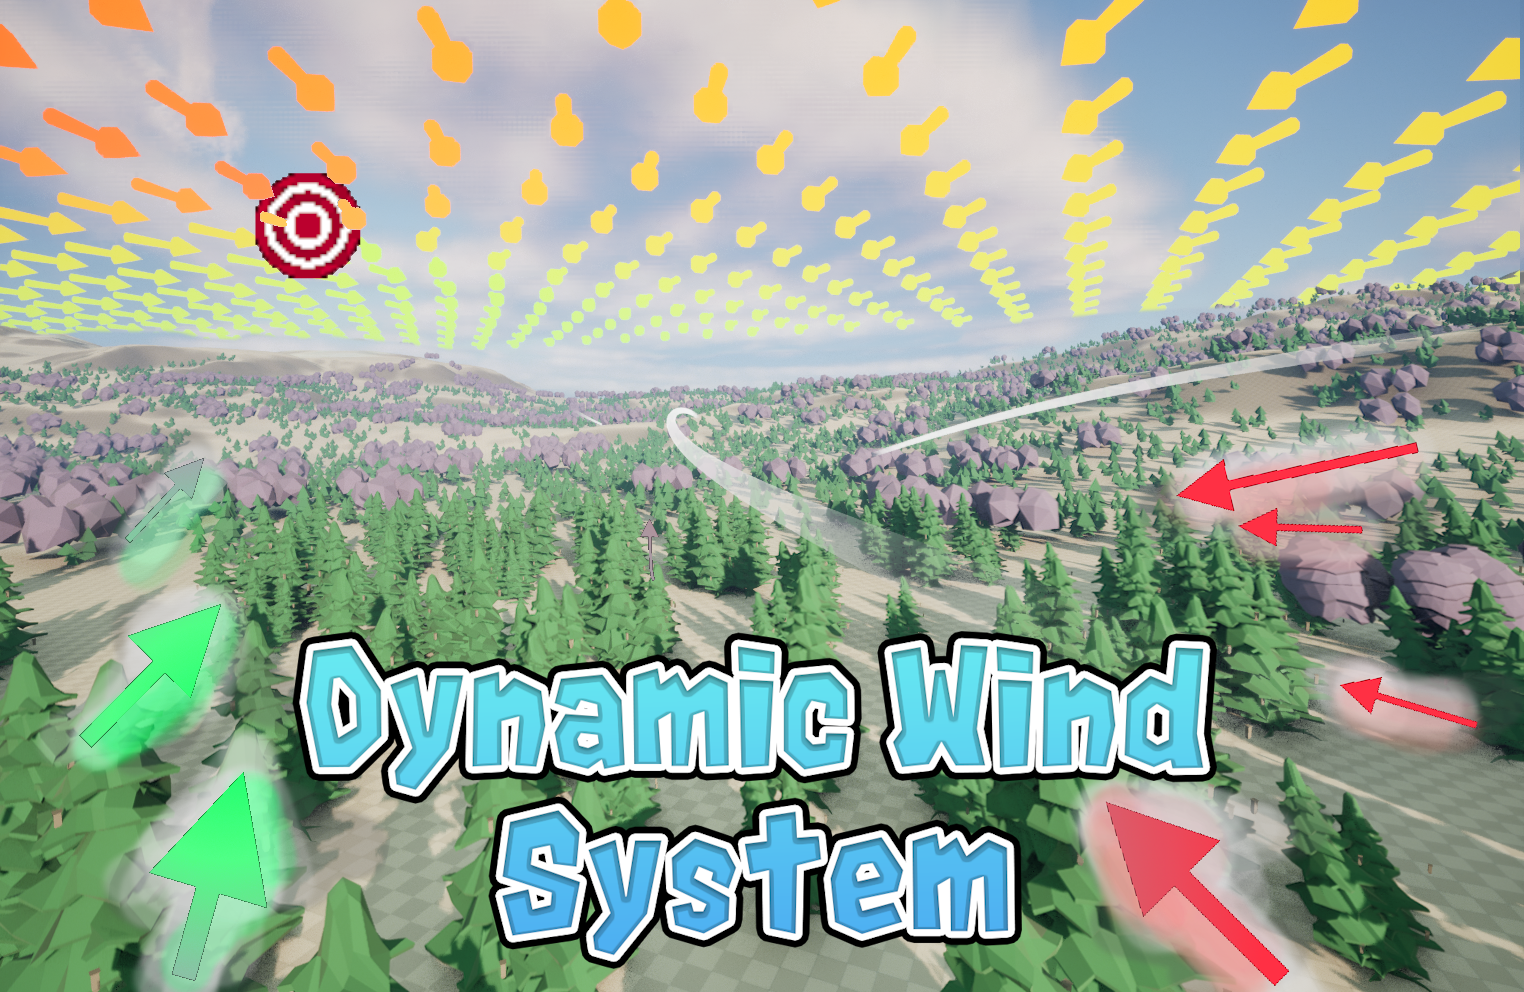
\includegraphics[width=1\textwidth]{Ressources/Thumbnail.png}
\end{figure}

% \begin{center}
%     \rule{.4\textwidth}{0.4pt}
% \end{center}
% \vspace*{12pt}
% \begin{figure}[H]
%     \centering
%     \begin{subfigure}{0.45\textwidth}
%         \centering
%         \includegraphics[width=.5\textwidth]{Ressources/GaltouzLogo_v2.png}
%     \end{subfigure}\hspace*{0.1\textwidth}
%     \begin{subfigure}{0.45\textwidth}
%         \centering

%         \includegraphics[width=0.5\textwidth]{Ressources/Profile.png}
%     \end{subfigure}
% \end{figure}


\newpage

\subfile{Pages/0_Intro.tex} 
% -----------------------------------------------------------
% Content prepartion

\tableofcontents
\thispagestyle{empty}	
\setcounter{page}{1}
\pagenumbering{arabic}

\newpage

% -----------------------------------------------------------
\subfile{Pages/5_HowToUse.tex}
\subfile{Pages/1_PhysicalTheorie.tex} 
\subfile{Pages/2_MoveTheActors.tex} 
\subfile{Pages/3_ShaderComputations.tex}
\subfile{Pages/4_BeyondScope.tex}
\end{document}